\documentclass[tikz]{standalone}

\usepackage{tikz}
\usetikzlibrary{shapes.geometric, arrows}


\tikzstyle{start} = [minimum height=1cm]
\tikzstyle{box} = [rectangle, minimum width=1.25cm ,text width=1.9cm,minimum height=1.7cm,text centered, draw=black]
\tikzstyle{fgain} = [isosceles triangle,isosceles triangle apex angle=60,draw=black]
\tikzstyle{fbox} = [rectangle, minimum width=0.75cm,minimum height=0.75cm,text centered, draw=black]
\tikzstyle{foperation} = [circle, radius=0.2, minimum size=0.75cm,inner sep=0pt, draw=black]
\tikzstyle{stop} = [minimum height=1cm]

\begin{document}
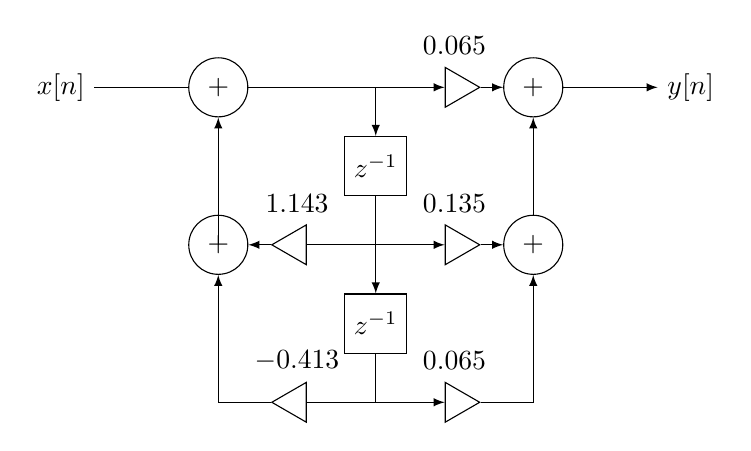
\begin{tikzpicture}[node distance=3cm]
    \node at (0,4) [start] (start) {$x[n]$};
    \node at (3,0) [fgain,rotate=180] (gain3) {};
    \node at (2,2) [foperation] (op2) {$+$};
    \node at (4,1) [fbox] (delai2) {$z^{-1}$};
    \node at (3,2) [fgain,rotate=180] (gain2) {};
    \node at (2,4) [foperation] (op1) {$+$};
    \node at (4,3) [fbox] (delai1) {$z^{-1}$};
    \node at (5,4) [fgain] (gain1) {} ;

    \node[above of=gain1,node distance=1.5em]{$0.065$};
    \node[above of=gain2,node distance=1.5em]{$1.143$};
    \node[above of=gain3,node distance=1.5em]{$-0.413$};
    

    \node at (5,0) [fgain] (gain22) {};
    \node at (6,2) [foperation] (op22) {$+$};
    \node at (5,2) [fgain] (gain21) {};
    \node at (6,4) [foperation] (op21) {$+$};
    \node at (8,4) [stop] (stop) {$y[n]$};
    \node[above of=gain21,node distance=1.5em]{$0.135$};
    \node[above of=gain22,node distance=1.5em]{$0.065$};
    
    
    \draw[-] (start) -- (op1);
    \draw[->,>=latex] (op1) -- (gain1);
    \draw[->,>=latex] (op1) -| (delai1);
    \draw[->,>=latex] (gain1) -- (op21);
    \draw[->,>=latex] (delai1) -- (delai2);
    \draw[->,>=latex] (delai1) |- (gain21);
    \draw[->,>=latex] (gain21) -- (op22);
    \draw[-] (delai1) |- (gain2);
    \draw[->,>=latex] (gain2) -- (op2);
    \draw[-] (delai2) |- (gain3);
    \draw[->,>=latex] (gain3) -| (op2);
    \draw[->,>=latex] (delai2) |- (gain22);
    \draw[->,>=latex] (gain22) -| (op22);
    \draw[->,>=latex] (op2) -| (op1);
    \draw[->,>=latex] (op22) -- (op21);
    \draw[->,>=latex] (op21) -- (stop);

    \end{tikzpicture}
\end{document}